% !TEX root = Thesis.tex

\section{Case Studies}

\subsection{Interview Technique}
%TODO evtl kürzer fassen
In order to complement theoretical findings from literature research, expert interviews have been conducted. A structure for the interviews has been defined (see appendix). In this way, statements from different experts can be compared and evaluated, which allows for a comprehensive review. Even though interviewees may share their native language (German) with the interviewer, interviews have always been conducted in English. Thus, any inaccuracies that may occur during translating the statements were prevented and comparability of interviews has been improved.

The interviews were held remotely, either via an Internet VoIP-Service such as Skype, or via using WebEx, the standard communication platform used at T-Systems when interviewing employees of this company. Considering the often tight schedules of experts in their fields, the duration of interviews was limited to 45 minutes.

To further document the interviews and the steps leading up to them as well as the steps of refinement that follow, a process (see figure \ref{fig:Intprocess}) has been defined and adhered to. 

%TODO Bild aktualisieren!!
\begin{figure}[htb]
	\centering
	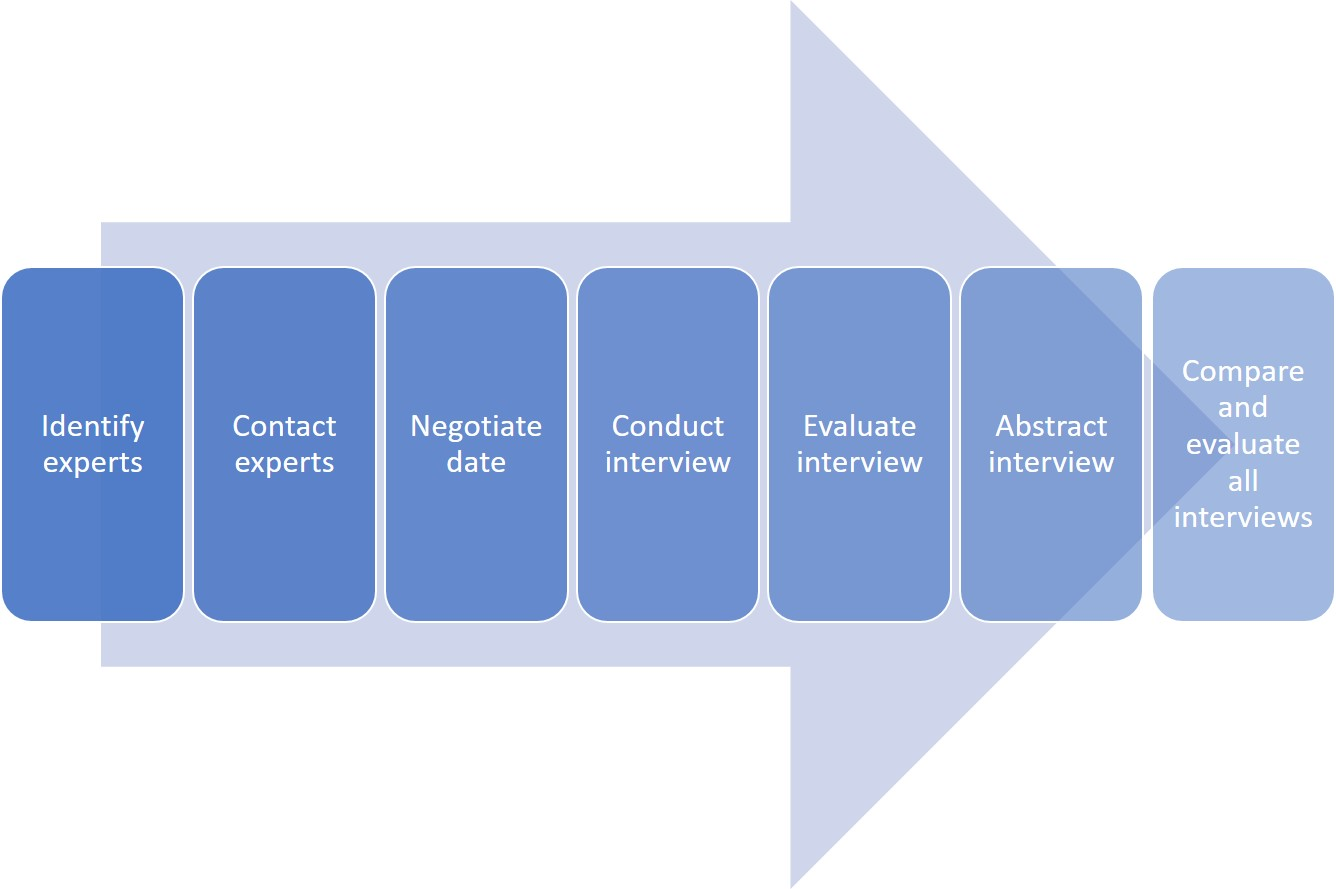
\includegraphics[width=0.7\textwidth]{Pictures/Interview_process}
	\caption{Interview process}
	\label{fig:Intprocess}
\end{figure}

\paragraph{Identify experts} The experts are identified by conducting a network-based search. Initial contacts are asked to identify persons they consider an expert on the topic, who are in turn asked to provide further contacts.
\paragraph{Contact experts} Initial contact to the expert is established via an email sent by the expert's contact. Included is a standard email explaining the topic, duration and process of the interview and providing the researchers' contact details.
\paragraph{Negotiate date} Once the expert has agreed to participate in the interview, the researcher contacts them directly in order to set up date, time and method of communication for the interview. Note that all interviews are conducted using at least voice-based communication. Video can be added to further facilitate the communication between the expert and the researcher.
\paragraph{Conduct interview} The interviews are conducted in five phases with defined leading questions. This means, the leading questions will be asked, but the researcher will also ask further questions as appropriate to the course of the interview. These phases are:
\begin{itemize}
	\item Introduction
	\item Offshoring Experiences in the USA
	\item Offshoring Experiences in Germany
	\item Comparison of Experiences in Germany and the USA
	\item Finalization
\end{itemize}
During the interview, audio has been recorded. The audio files form the primary source of knowledge gained from the experts.


\paragraph{Evaluate interview} The recordings are evaluated and any important passages are noted. These evaluations are added to the appendix.

\paragraph{Abstract interview} For each interview, an abstract is developed. The abstracts are included in the thesis.

\paragraph{Compare and evaluate all interviews} Finally, an overview and comparison of all interviews is generated to derive common statements and areas of disagreement.


\subsection{Case Study Title 1}

\subsubsection{Background}
\subsubsection{Results of Interview}
\subsubsection{Conclusions}
\subsection{Case study Title 2}
\subsubsection{Background}
\subsubsection{Results of Interview}
\subsubsection{Conclusions}


\subsection{Summary and Evaluation}
